\section{Deterministic Finite Automata}

\textbf{Finite automaton}, or \textbf{finite-state machine} shares with a real computer the fact that it has a ``central processing unit'' of fixed, finite capacity. It receives its input as a string, delivered to it on an input tape. It delivers no output at all, except an indication of whether or not the input is considered acceptable. It is, in other words, a language recognition device.

What makes the finite automaton such a restricted model of real computers is the \textit{complete absence of memory} outside its fixed central processor.

\begin{figure}[h!]
  \centering
  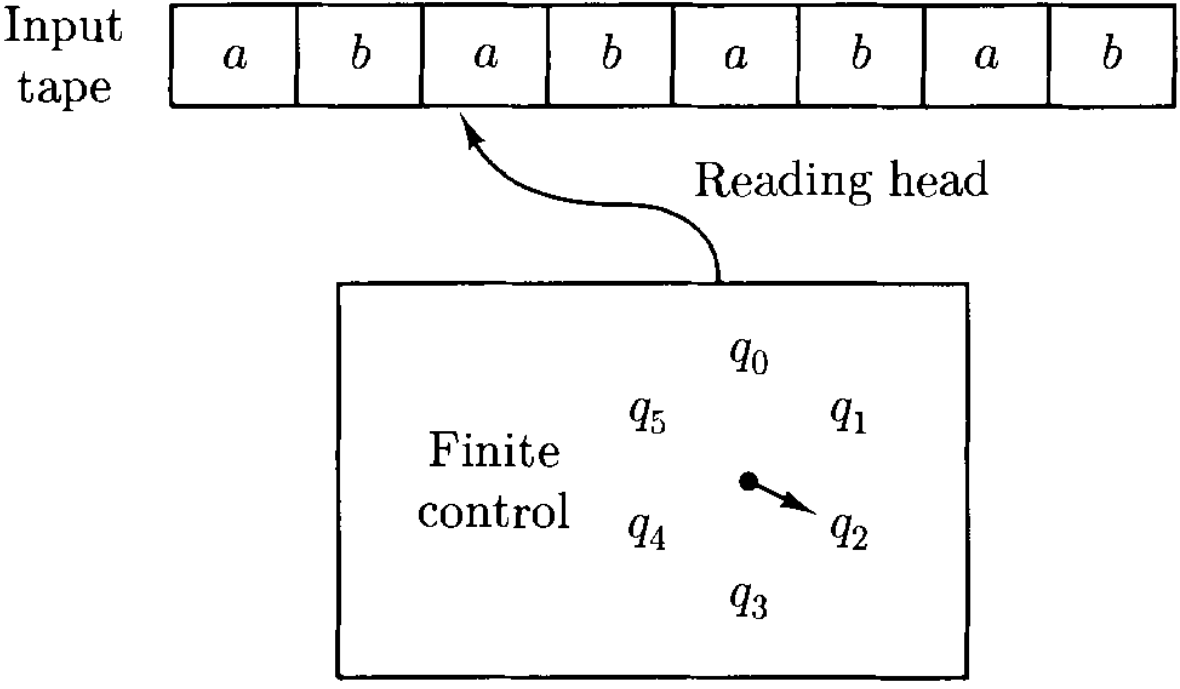
\includegraphics[width=.5\textwidth]{img/Fig2.1.png}
  \caption{Finite Automata}
\end{figure}

\begin{multicols}{2}
\setlength{\columnsep}{1.5cm}
\setlength{\columnseprule}{0.2pt}
  Let's describe the operation of a finite automaton in more detail. 
  \begin{itemize}
    \item Strings are fed into the device by means of an \textbf{input tape}, which is divided into squares, with one symbol inscribed in each tape square (see Figure 1).
    \item The main part of the machine itself is a ``black box'', with innards that can be, at any specified moment, in one of a finite number of distinct internal states.
    \item The black box -called the \textbf{finite control}- can sense what symbol is written at any position on the input tape by means of a movable \textbf{reading head}.
    \item Initially, the reading head is placed at the leftmost square of the tape and the finite control is set in a designated \textbf{initial state}.
    \item At regular intervals the automaton reads one symbol from the input tape and then enters a new state that \textit{depends only on the current state and the symbol just read}.
    \item After reading an input symbol, the reading head moves one square to the right on the input tape so that on the next move it will read the symbol in the next tape square. This process is repeated again and again; a symbol is read, the reading head moves to the right, and the state of the finite control changes. Eventually the reading head reaches the end of the input string.
    \item The automaton then indicates its approval or disapproval of what
    it has read by the state it is in at the end: if it winds up in one of a set of \textbf{final states} the input string is considered to be \textbf{accepted}.
    \item The language accepted by the machine is the set of strings it accepts.
  \end{itemize}
\end{multicols}

\begin{definition}{}
  A \textbf{deterministic finite automaton} is a quintuple $M = (K, \Sigma, \delta, s, F)$ where
  \begin{itemize}
    \item $K$ is a finite set of \textbf{states}
    \item $\Sigma$ is an alphabet,
    \item $s \in K$ is the \textbf{initial state}
    \item $F \subseteq K$ is the set of \textbf{final states}
    \item $\delta$, the \textbf{transition function}, is a function from $K \times \Sigma$ to $K$. 
  \end{itemize}
\end{definition}

The \textbf{configuration} of the machine is the \textit{current state and the unread part of the input string}, i.e., a configuration is an element of $K \times \Sigma^*$.

The binary $\vdash_M$ (yields) relation holds between two configurations of $M$ if and only if the machine can pass from one configuration to another one as a result of a single move. Let $(q, w)$ and $(q',w')$ be two configurations of $M$. Then $(q, w) \vdash_M (q', w')$ if and only if $w = aw'$ for some $a \in \Sigma$ and $q' = \delta(q, a)$. $(q, w) \vdash_M (q', w')$ reads $(q, w)$ \textbf{yields} $(q', w')$ in \textbf{one step}. Note that $\vdash_M$ is a function from $K \times \Sigma^+$ to $K \times \Sigma^*$, hence, for every configuration except $(q, e)$ there exists a uniquely determined next configuration.

$\vdash^*_M$ is the \textbf{reflexive transitive closure} of $\vdash_M$. $(q, w) \vdash^*_M (q', w')$ reads $(q, w)$ \textbf{yields} $(q', w')$. A string $w \in \Sigma^*$ is \textbf{accepted} by $M$ if and only if $(s, w) \vdash^*_M (f, e)$ for some $f \in F$. The \textbf{language} of $M$, $L(M)$, is the set of strings \textit{accepted} by $M$.

\begin{example}{}
  Let $M$ be the deterministic finite automaton $(K, \Sigma, \delta, s, F)$, where
  \begin{multicols}{2}
    \begin{itemize}
      \item $K = \left\{ q_0, q_1 \right\}$
      \item $\Sigma = \left\{ a, b \right\}$
      \item $s = q_0$
      \item $F = \left\{ q_0 \right\}$
    \end{itemize}
  \end{multicols}
  and $\delta$ is the function tabulated below.
  \begin{center}
    \begin{tabular}{c|c|c}
      $q$      & $\sigma$ & $\delta(q, \sigma)$  \\ 
      \hline
      $q_0$ & $a$    & $q_0$             \\
      $q_0$ & $b$    & $q_1$             \\
      $q_1$ & $a$    & $q_1$             \\
      $q_1$ & $b$    & $q_0$            
    \end{tabular}
  \end{center}

  It is then easy to see that $L(M)$ is the set of all strings in $\left\{ a, b \right\}^*$ that have an even number of $b$'s. For $M$ passes from state $q_0$ to $q_1$ or from $q_1$ back to $q_0$ when $a$ $b$ is read, but $M$ essentially ignores $a$'s, always remaining in its current state when an $a$ is read. Thus $M$ counts $b$'s modulo 2, and since $q_0$ (the initial state) is also the sole final state, $M$ accepts a string if and only if the number of $b$'s is even.
  
  If $M$ is given the input $aabba$, its initial configuration is $(q_0, aabba)$. Then 
  \begin{align*}
    (q_0, aabba) &\vdash_M (q_0, abba)\\
    &\vdash_M (q_0, bba)\\
    &\vdash_M (q_1, ba)\\
    &\vdash_M (q_0, a)\\
    &\vdash_M (q_0, e)
  \end{align*}
  Therefore $(q_0, aabba) \vdash^*_M (q_0, e)$, and so $aabba$ is accepted by $M$.
\end{example}

\begin{figure}[h!]
  \centering
  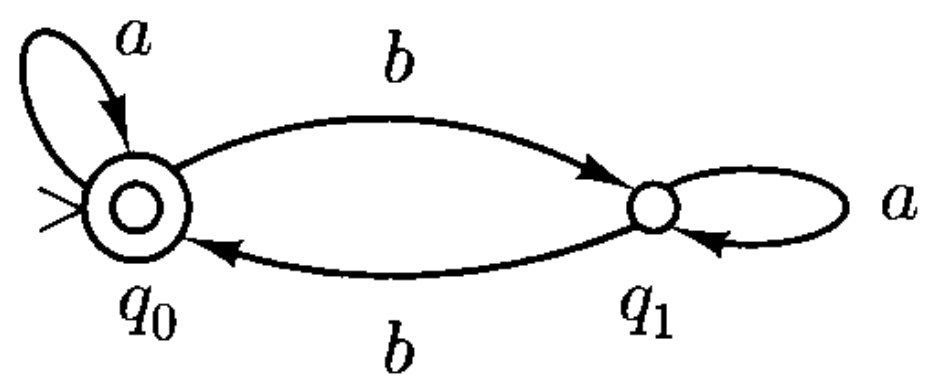
\includegraphics[width=.3\textwidth]{img/Fig2.2.png}
  \caption{State Diagram}
\end{figure}
The tabular representation of the transition function used in this example is not the clearest description of a machine. We generally use a more convenient graphical representation called the \textbf{state diagram} (Figure 2).
